% utf-8 ru, unix eolns
\documentclass[14pt,a4paper,oneside]{extarticle}
    \righthyphenmin=2 %минимально переносится 2 символа %%%
    \sloppy

\renewcommand{\baselinestretch}{1.5}

% Рукопись оформлена в соответствии с правилами оформления 
% электронной версии авторского оригинала, 
% принятыми в Издательстве МГТУ им. Н.Э. Баумана.

\usepackage{geometry} % А4, примерно 28-31 строк(а) на странице 
    \geometry{paper=a4paper}
    \geometry{includehead=false} % Нет верх. колонтитула
    \geometry{includefoot=true}  % Есть номер страницы
    \geometry{bindingoffset=0mm} % Переплет    : 0  мм
    \geometry{top=20mm}          % Поле верхнее: 20 мм
    \geometry{bottom=25mm}       % Поле нижнее : 25 мм 
    \geometry{left=25mm}         % Поле левое  : 25 мм
    \geometry{right=25mm}        % Поле правое : 25 мм
    \geometry{headsep=10mm}  % От края до верх. колонтитула: 10 мм
    \geometry{footskip=20mm} % От края до нижн. колонтитула: 20 мм 

\usepackage{cmap}
\usepackage[T2A]{fontenc} 
\usepackage[utf8x]{inputenc}
\usepackage[english,russian]{babel}
\usepackage{misccorr}

\usepackage{amsmath}
\usepackage{amsfonts}
\usepackage{amssymb}

%\usepackage{cm-super} %человеческий рендер русских шрифтов

\setlength{\parindent}{1.25cm}  % Абзацный отступ: 1,25 см
\usepackage{indentfirst}        % 1-й абзац имеет отступ

\usepackage{setspace}   

\onehalfspacing % Полуторный интервал между строками

\makeatletter
\renewcommand{\@oddfoot }{\hfil\thepage\hfil} % Номер стр.
\renewcommand{\@evenfoot}{\hfil\thepage\hfil} % Номер стр.
\renewcommand{\@oddhead }{} % Нет верх. колонтитула
\renewcommand{\@evenhead}{} % Нет верх. колонтитула
\makeatother

\usepackage{fancyvrb}

\usepackage[nounderscore]{syntax} %для поддержки рбнф
%\setlength{\grammarindent}{12em} %устанавливает нужный отступ перед ::=
\setlength{\grammarparsep}{6pt plus 1pt minus 1pt}  %сокращает расстояние между правилами


\usepackage[pdftex]{graphicx}  % поддержка картинок для пдф
\graphicspath{ {./pictures/} }
\usepackage{rotating}
\usepackage{graphicx}
%\DeclareGraphicsExtensions{.jpg,.png}

\renewcommand{\labelenumi}{\theenumi.} %меняет вид нумерованного списка

\usepackage{perpage} %нумерация сносок 
\MakePerPage{footnote}

\usepackage[all]{xy} %поддержка графов

\usepackage{listings} %листинги
\renewcommand{\lstlistingname}{Листинг}
\lstset{
  basicstyle=\small,
  breaklines=true
  }

\usepackage{url}


\usepackage{tikz} %для рисования графиков
\usepackage{pgfplots}

\usepackage{rotating}

\usepackage{ccaption}%изменяет подпись к рисунку
\makeatletter 
\renewcommand{\fnum@figure}[1]{Рисунок~\thefigure~---~\sffamily}
\makeatother





\begin{document}
\pgfplotsset{compat=1.8}

\thispagestyle{empty}
\newpage
{
\centering


\textbf{
МОСКОВСКИЙ ГОСУДАРСТВЕННЫЙ ТЕХНИЧЕСКИЙ УНИВЕРСИТЕТ ИМЕНИ Н. Э. БАУМАНА \\
Факультет информатики и систем управления \\
Кафедра теоретической информатики и компьютерных технологий}
\bigskip
\bigskip
\bigskip
\bigskip
\bigskip
\bigskip
\bigskip

\vfill

Курсовой проект \\
по курсу <<Конструирование компиляторов>>

\bigskip

{\large <<Препроцессор синаксического сахара для языка Scheme>>}
\bigskip

\vfill



\hfill\parbox{4cm} {
Выполнил:\\
студент ИУ9-101 \hfill \\
Выборнов А. И.\hfill \medskip\\
Руководитель:\\
Дубанов А. В.\hfill
}


\vspace{\fill}

Москва \number\year
\clearpage
}


\tableofcontents

\clearpage

\section*{Введение}
\addcontentsline{toc}{section}{Введение}
    В современном мире всё больший вес приобретают социальные медиа (преимущественно социальные сети). Их главное отличие от традиционных медиа (газеты, тв) заключается в том, что контент порождается тысячами и миллионами людей. Социальные медиа не заменяют традиционные новостные источники, а дополняют их. Они могут служить полезным социальным датчиком того, насколько популярна история (тема) и как долго. Часто обсуждения в социальных медиа основаны на событиях из новостей и, наоборот, социальные медиа влияют на новостные события.

    Одной из самых популярных социальных сетей является Twitter - социальная сеть для публичного обмена сообщениями. Главной особенностью Twitter является малый размер сообщений (140 символов), называемых твитами. Часто твиты являют собой описание, происходящего прямо сейчас события, отклик на него.

    ...

    Выявление связи между сообщениями твиттера (твитов) и новостями позволит как расширить информативность твитов, так и обогатить новости.

    ...

    Преимущества расширения новости с помощью твитов: определение отношения аудитории к новости, дополнительные признаки для тематической классификации новостей, дополнительная информация для аннотирования новостей.

    Современные методы обработки естественного языка хорошо работают, используя большой массив текста в качестве входных данных, однако, они становятся неэффективными, когда применяются на коротких текстах, таких как твиты. Существенным преимуществом расширения твита с помощью новости является появляющаяся возможность использования большого количества методов обработки естественного языка (Natural Language Processing).

    ...


    Данная работа ставит целью исследование и разработку методов автоматического установления связей между сообщениями твиттера и новостными статьями.

    {\color{red} Не существует стандартных решений. и есть считанное количество статей. На основе этих статей будет сделана попытка построить pipeline для получения подобной взаимосвязи.}

    \clearpage


\section{Обзор литературы}
    В рамках предварительного исследования были разобраны несколько статей \cite{linking_base} \cite{linking_news_media} \cite{bridging}. Ниже приводится краткое изложение основных идей, описанных в выбранных статьях.    
    
    \subsection{Linking Tweets to News: A Framework to Enrich Short Text Data in Social Media}
        \subsubsection{Перевод аннотации}
        Многие современные методы обработки естественного языка~(NLP\footnote{Natural Language Processing}) хорошо работают с большой массив текста в качестве входных данных.
        Однако они очень неэффективными при работе с короткими текстами (к примеру твиты).
        Преодоление этой проблемы мы видим в нахождении соответствующего твиту новостного документа.
        Решение этой задачи требует хорошего моделирования семантики коротких текстов.

        Основной вклад статьи двойной:
        \begin{enumerate}
            \item представлено решение задачи нахождения взаимосвязи между твитами и новостями, из этого могут извлечь выгоду многие NLP задачи;
            \item в отличие от предыдущих исследований, которые фокусируются на лексических особенностях коротких текстов~(информация о связи текст-слово), мы предлагаем взаимосвязь, основанную на модели скрытой переменной, которая моделирует корреляцию между короткими текстами~(информация о связи текст-текст). Необходимость этого обоснована наблюдением: твит обычно покрывает только один аспект события.
        \end{enumerate}
        
        Мы покажем, что c помощью особенных признаков твита~(хэштегов) и особых признаков новостей~(именнованных сущностей\footnote{Какой-то кривой перевод, найдо найти получше. In data mining, a named entity is a phrase that clearly identifies one item from a set of other items that have similar attributes.}) а также временн\'{ы}х ограничений, мы можем получить взаимосвязь текст-текст, и, таким образом, дополнить семантическую картину короткого текста.
        Наши эксперименты показывают значительное преимущество нашей новой модели над baseline\footnote{Как перевести?}.

        \subsubsection{Идея статьи}
        Современные методы обработки естественного языка плохо работают с короткими текстами. Для преоболения этого к твитам привязываются соответствующие новости. 

        Для формирования обучающей выборки, были выбраны твиты, которые имели ссылки на новости, опубликованные новостными агенствами (CNN или NYT) в тот же период.
        
        Как показано в статье~\cite{long_to_short}, добавление к твиту содержимого веб-страницы, ссылка на которую включена в этот твит, повышает {\color{red} purity score} их кластеризации с 0.280 до 0.392.

        Модели со скрытой переменной хорошо подходят для отображения коротких текстов в плотный малоразмерный вектор.
        В рамках решения задачи была применена модель со скрытой переменной, которая называется WTMF~(Weighted Textual Matrix Factorization, подробное описание\cite{wtmf}), к твитам и к новостям. Модель была протестирована на двух схожих наборах данных из небольших сообщений. Как результат - используемая модель с большим запасом превзошла и LSA~(Latent Semantic Analysis) и LDA~(Latent Dirichelet Allocation). Эта модель позволила добавить информацию об отсутствующих словах в твит (модель WTMF добавляет более 1000 фичей к твиту, LDA лишь 14). Недостатком WTMF является то, что порождается только связь текст-слово, без учёта взаимосвязи между короткими текстами.
        
        Ввиду разреженности исходных данных, возникает ещё одна проблема: твит обычно отражает, только один аспект события.

        Полученный подход не учитывает следующих характеристик, которым обладает исходная выборка:
        \begin{enumerate}
            \item Хэштеги, которые являются прямым указанием на смысл твита.
            \item {\color{red} Named entities} новостей. Из новостей можно с высокой точностью извлекать {\color{red} named entities}, используя инструменты для NER~(Named Entity Recognition). Если несколько текстов содержат схожие {\color{red} named entities} они наверняка описывают одно и тоже событие.
            \item Информация о времени публикации для твитов и новостей. Если несколько текстов опубликованы примерно в одно и то же время, то велик шанс, что они описывают одно и тоже событие
        \end{enumerate}
        В статье описывается решение проблемы поиска взаимосвязи между текстами, с использованием описанных выше характеристик. Два связанных текста, должны иметь схожий скрытый вектор (семантическая модель твита достраивается из схожих твитов).

        Это дополнительная информация была добавлена в модель WTMF. Было также показано различное влияние на связь текст-текст жанра твита и жанра новости. Был получен на порядок более лучший результат чем при использовании исходной WTMF модель.

    \subsection{Linking Online News and Social Media}
        \subsubsection{Перевод аннотации}
            Многое из того, что обсуждается в социальных медиа вдохновлено событиями, описанными в новостях и, наоборот, социальные медиа предоставляют механизм, позволяющий влиять на новостные события.
            Мы обращаемся к следующей задаче: по новости, найти в социальных сетях высказывания, которые неявно на неё ссылаются.
            Используется трехступенчатый подход: сначала получаются несколько моделей запросов по исходной статье, затем модели используются для получения высказываний из индекса целевого социального медиа, результатом являются несколько ранжированных списков, которые объединяются с использованием особой техники слияния данных.
            Модель запроса создаётся как на основе структуры статьи, так и на основе явно связанных со статьей высказываний из социальных медиа.
            Для борьбы с дрейфом запроса\footnote{Порождение менее подходящего запроса.} при большого объёме используемого текста (либо в новости, либо в явно связанных высказываниях из социальных медиа), предлагается основанный на графике метод для выбора отличительных условий.

            В нашей экспериментальной оценки для порождения моделей запросов, использованы данные из Twitter, Digg, Delicious\footnote{Веб-сайт, бесплатно дающий зарегистрированным пользователям услугу хранения и публикации закладок на страницы Всемирной сети.}, the New York Times Community, Wikipedia и блогосферы.
            Показано, что другие модели запросов, основанные на различных источниках данных, не только обеспечивают дополнительную информацию, но и влияют на получение различных высказываний из социальные медиа по нашему целевому индексу.
            Как следствие, методы слияния данных приводят к значительному повышению производительности в сравнении с индивидуальными подходами.
            Показано, что основанный на графике метод выделения условий помог улучшить как эффективность, так и продуктивность.

    \subsection{Bridging Vocabularies to Link Tweets and News}
        \subsubsection{Основная идея}
            Значительную сложность при решении проблемы связывания твитов с новостями преимущественно вызывают малый размер твита и различия в словарях: в твитах используются аббревиатуры, неформальный язык, сленг, в новостях, напротив, используется литературный язык. Также твиты очень зашумлены и не содержать полезного содержимого.

            Твиттер предлагает хештэги, как механизм для категоризации твитов. Но этот подход далеко не совершенен, так как не только далеко не все записи содержат хештеги, но и записи содержащие хeштеги обладают рядом проблем. Такими как: хeштег не содержит информацию о событии, хeштег сформулирован в слишком общей форме, твит содержит несколько хештегов. Из этого делается вывод, что использование только хештегов приведёт к низкому качеству связывания твитов с новостями.

            Предлагается следующий подход:
            Используется LDA для построения моделей тем поверх новостей. Затем среди твитов ищутся наиболее близкие к конкретному топику. Из полученных твитов извлекаются слова, которые служат ``мостом'' к другим твитам.
    \subsection{TwitterStand: News in Tweets}
        Формирование дайджеста новостей на основе твиттера, не очень коррелирует с темой. Но возможно в статье есть хорошие идеи, которые помогут с решением задачи.


\section{Дополнительная литература}
    \subsection{Gibberish, Assistant, or Master? Using Tweets Linking to News for Extractive Single-Document Summarization}
    \subsection{Detecting Event-Related Links and Sentiments from Social Media Texts}
    \subsection{Определение тематической направленности текстового содержимого микроблогов}
    \subsection{Разработка сервиса извлечения мнений}
    

\section{Полезные ссылки}
    \begin{itemize}
        \item Твиттер NYT: https://twitter.com/nytimes (20млн подписчиков, 200тыс твитов)
        \item Крайне отстойная статья на тему: http://cyberleninka.ru/article/n/issledovanie-otklika-polzovateley-twitter-na-novosti-iz-smi
        \item Идея для формирования train: http://techcrunch.com/2013/08/19/twitter-related-headlines/
    \end{itemize}
\clearpage

\section{Описание реализации}
    Из предложенных статей единственная полноценная - Linking tweets to news by guo.

    \subsection{Linking Tweets to News: A Framework to Enrich Short Text Data in Social Media}
        \subsubsection{Построение датасетов}
            За один и тот же промежуток выкачиваем твиты с помощью stream api, новости с помощью rss.

            Твит задаётся кортежем: (time, author, text). Новость задаётся кортежем: (time, title, summary, url).

            Train/test множества формируем из твитов, которые содержат единственную ссылку на новость, из выкаченных нами ранее, и не совпадают с заголовком новости.

        \subsubsection{Evaluation}
            Используем метрику $ATOP$ (метрика подробно описана в \cite{steck_recommender}).
            Рассмотрим что означает эта метрика в применении к нашей задаче (я немного модифицировал метрику, для более простого описания, полученная метрика полностью совпадает с описанной метрикой).
            Пусть $T$ - это множество твитов, $N \in \mathbb{N}$ - размер рассматриваемого топа новостей для твита (могут быть все новости вообще), $k < N \in \mathbb{N}$.
            $TOPK_t(k) = 1$, если твит $t \in T$ соответствует хотя бы одной новости в top-k результатов, иначе $TOPK_t(k) = 0$
            $$TOPK(k) = \dfrac {\sum_{t \in T} TOPK_t(k)} {|T|},$$
            $$ATOP = \dfrac{\sum_{k=1}^N TOPK_t(k)}{N} = \dfrac{1}{|T| * N} \sum_{k=\overline{1,N}, ~t \in T} TOPK_t(k).$$

            Значения метрики $ATOP$ лежат на отрезке $[0,1]$. Чем ближе $ATOP$ к $1$ тем лучше.

        \subsubsection{WTMF}
            WTMF - модель применяемая для анализа схожести между короткими текстами \cite{wtmf}. Модель рассматривает отсутствующие в тексте слова как признаки короткого текста. Отсутсвующие слова это все слова корпуса рассматриваемых текстов за исключением слов из рассматриваемого короткого текста. Отсутствующие слова являются негативным сигналом для смысла коротких текстов.

            WTMF похож на SVD, но использует не разложение, а непосредственный расчёт каждой ячейки. Модель раскладывает матрицу $X \sim P^TQ$.

            Корпус рассматривается как матрица $X$ размера $M \times N$: строки - это слова (всего $M$), столбцы - короткие тексты (всего $N$), ячейки - мера tf-idf. 
            Как показано на рисунке~\ref{pic:wtmf} матрица $X$ приближается произведением двух матриц $P$ размера $M \times K$ и $Q$ размера $K \times N$.

            \begin{figure}[h!]
                \center
                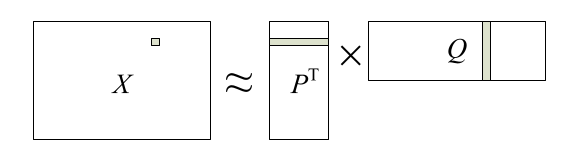
\includegraphics[scale=0.45]{wtmf.png}
                \caption{wtmf}
                \label{pic:wtmf}
            \end{figure}

            Каждый текст $s_j$ представлен в виде вектора $Q_{\cdot,j}$ размерности $K$, каждое слово $w_i$ представлено в виде вектор $P_{i,\cdot}$. Когда их скалярное произведение $X_{ij}$ близко к нулю, то мы считаем, что это отсутствующее слово.

            Задачей модели является минимизация целевой функции ({\color{red}$\lambda$ - регуляризирующий член}, матрица W определяет вес каждого элемента матрицы X):
            $$\sum_i \sum_j W_{ij} (P_{i,\cdot} \cdot Q_{\cdot,j} - X_{ij})^2 + \lambda ||P||^2_2 + \lambda ||Q||^2_2.$$

            Для получения векторов $P_{i,\cdot}$ и $Q_{\cdot,j}$ используется алгоритм описанный в статье~\cite{matrix_approximation}. Сначала P и Q инициализируются случайными числами. Затем запускается итеративный пересчёт P и Q по следующим формулам (эффективный способ расчёта описан в \cite{steck_recommender}):
            $$P_{i, \cdot} = (Q W'_i Q^T + \lambda I)^{-1} Q W'_i X_{i,\cdot}^T,$$
            $$Q_{\cdot, j} = (P W'_j P^T + \lambda I)^{-1} P W'_j X_{j,\cdot}.$$
            Здесь $W'_i = diag(W_{i, \cdot})$ - диагональная матрица полученная из $i$-ой строчки матрицы $W$, аналогично $W'_j = diag(W_{\cdot, j})$ - диагональная матрица полученная из $j$-ого столбца.

            Определим матрицу W следующим образом:
            \begin{gather}
                W_{ij} = 
                \begin{cases}
                    1, ~~if~X_{ij} \neq 0, \nonumber \\
                    w_m, ~~otherwise. 
                \end{cases},
            \end{gather}
            где $w_m$ положительно и $w_m << 1$.

        \subsubsection{Построение связей текст-текст}
            Твиты связываются с помощью хэштегов, named entities и времени.

            Связь твитов с помощью хэштэгов. Сначала извлекаем все хэштеги из твитов, затем превращаем в хэштеги все слова во всех твитах, которые совпали с ранее извлечёнными хэштэгами. Для каждого твита и для каждого хэштэга извлекаем $k$ твитов, которые содержат этот этот хэштег, если хэштег появлялся в более чем $k$ твитах берём $k$ твитов наиболее близких во времени к исходному.

            Связь твитов с помощью named entities. Применяем методы NER к новостным summary и получаем множество named entities. Затем применяем тот же подход, что и к хэштегам, сначала превращаем в NE слова из твитов, которые совпали с полученными NE, а затем получаем $k$ связей для каждого твита.

            Связь твитов с помощью времени. Аналогично вышеописанному для каждого твита выбираем $k$ связей с наиболее схожими твитами в окрестности 24 часов. Наиболее близкие находятся с помощью косинусной меры, расчитываемой для векторов из таблицы X.

            Новости связываются только по времени.
        \subsubsection{WTMF-G}
            Добавление связей текст-текст в WTMF происходит с помощью влияния на regularization term. Для каждой пары связанных текстов $j_1$ и $j_2$:
            $$\lambda = \delta \cdot (\dfrac{Q_{\cdot,j_1}\cdot Q_{\cdot,j_2}}{|Q_{\cdot,j_1}|| Q_{\cdot,j_2}|}-1)^2,$$
            коэффициент $\delta$ задаёт степень влияния связей текст-текст.

            Полученная модель и называется WTMF-G (WTMG on graphs).

            Alternating Least Square используемый в \cite{steck_recommender} не применим из-за нового regularization term, который зависит от $|Q_{\cdot,j}|$ ({\color{red} по-хорошему нужно понять почему}). Для того, чтобы мы могли применить ALS мы вводим упрощение: длина вектора $Q_{\cdot,j}$ не изменяется во время итерации. Получаем уравнения:
            $$P_{i, \cdot} = (Q W'_i Q^T + \lambda I)^{-1} Q W'_i X_{i,\cdot}^T,$$
            $$Q_{\cdot, j} = (P W'_j P^T + \lambda I + \delta  L_j^2 Q_{\cdot,n(j)} diag(L^2_{n(j)})Q_{\cdot,n(j)}^T)^{-1}   (P W'_j X_{j,\cdot} + \delta  L_j Q_{\cdot,n(j)} L_{n(j)}).$$
            В этих формулах $n(j)$~---~список связанных текстов с текстом $j$. $Q_{\cdot,n(j)}$~---~матрица, состоящая из связанных векторов для $Q_{\cdot, j}$. $L_j$ - длина вектора $Q_j$ на начало итерации, $L_n(j)$~---~вектор длин векторов связанных с $j$ i.e. $Q_{\cdot,n(j)}$, полученный на начало итерации.
            


\section{Формирование датасетов}
    Для формирования датасетов нужно сделать:
    \begin{enumerate}
        \item Выбрать источники данных.
        \item Выбрать формат хранения.
        \item Выбрать БД, для записи результата.
        \item Написать отказоустойчивый консьюмер.
        \item В течение длительного времени собрать данные.
    \end{enumerate}

    Предлагаю выбор формата хранения и БД отложить до тех пор, пока не будут получены все необходимые данные. А пока коллекционировать все возможные данные в текстовых файлах.

    В качестве источников данных 

    \subsection{Примерно что делал}
        Лог работы в raw формате :) будет много копипасты с используемых мануалов
 \begin{enumerate}
    \item Step 1: Getting Twitter API keys

        In order to access Twitter Streaming API, we need to get 4 pieces of information from Twitter: API key, API secret, Access token and Access token secret. Follow the steps below to get all 4 elements:

        Create a twitter account if you do not already have one.
        Go to https://apps.twitter.com/ and log in with your twitter credentials.
        Click "Create New App"
        Fill out the form, agree to the terms, and click "Create your Twitter application"
        In the next page, click on "API keys" tab, and copy your "API key" and "API secret".
        Scroll down and click "Create my access token", and copy your "Access token" and "Access token secret".
    \item 
    \end{enumerate}

\section{Используемое ПО}
    \subsection{tweepy}
        https://github.com/tweepy/tweepy

\clearpage
\begin{thebibliography}{0}
\addcontentsline{toc}{section}{Список литературы}
    \bibitem{linking_base} W. Guo, H. Li, H. Ji, and M. T. Diab. Linking tweets to news: A framework to enrich short text data in social media. - ACL, pages 239–249, 2013.
    \bibitem{linking_news_media} Manos Tsagkias, Maarten de Rijke, Wouter Weerkamp. Linking Online News and Social Media. - ISLA, University of Amsterdam.
    \bibitem{bridging} T. Hoang-Vu, A. Bessa, L. Barbosa and J. Freire. Bridging Vocabularies to Link Tweets and News. - International Workshop on the Web and Databases (WebDB 2014), Snowbird, Utah, US, 2014.
    \bibitem{twitterstand} J. Sankaranarayanan, H. Samet, B. Teitler, M. Lieberman, J. Sperling. TwitterStand: news in tweets. - 17th ACM SIGSPATIAL International Conference on Advances in Geographic Information Systems, 2009, Seattle, Washington.

    \bibitem{long_to_short} Ou Jin, Nathan N. Liu, Kai Zhao, Yong Yu, and Qiang Yang. 2011. Transferring topical knowledge from auxiliary long texts for short text clustering. In Proceedings of the 20th ACM international conference on Information and knowledge management.

    \bibitem{wtmf} Weiwei Guo and Mona Diab. 2012a. Modeling sentences in the latent space. In Proceedings of the 50th Annual Meeting of the Association for Computational Linguistics. 

    \bibitem{steck_recommender} Harald Steck. 2010. Training and testing of recommender systems on data missing not at random. In Proceedings of the 16th ACM SIGKDD International Conference on Knowledge Discovery and Data Mining.

    \bibitem{matrix_approximation} Nathan Srebro and Tommi Jaakkola. 2003. Weighted low-rank approximations. In Proceedings of the Twentieth International Conference on Machine Learning.

    \hrulefill

\end{thebibliography}

\end{document}

